\chapter{Introduction}\label{sec:intro-pomdp}
In this part of the manuscript, we show that direct reinforcement learning of decision tree policies for MDPs (cf. definition~\ref{def:mdp}), i.e. learning a decision tree that optimizes the RL objective (cf. definition~\ref{def:mdp-obj}) is often very difficult.
In particular, we provide some insights as to why it is so difficult and show that indirect imitation of a neural network policy (cf. section \ref{sec:imit}), while optimizing the imitation learning objective (cf. definition~\ref{def:il}) rather than the RL one, often yields very good tree policies in practice.

This first part of the manuscript is organized as follows.
In this chapter, we present Nicholay Topin and colleagues' framework for direct reinforcement learning of decision tree policies~\cite{topin2021iterative}.
In chapter \ref{sec:topin}, we reproduce experiments from~\cite{topin2021iterative} where we compare direct deep reinforcement learning (cf. section \ref{sec:drl}) of decision tree policies to indirect imitation of neural network policies with decision trees for the simple CartPole MDP~\cite{cartpole}.
In chapter \ref{sec:pomdp}, we show that this direct approach is equivalent to learning a deterministic memoryless policy for partially observable MDP (POMDP)\cite{POMDP,chap2}--which is a hard problem~\cite{littman1}--and show that this might be the main reason for failures.
In chapter \ref{sec:pomdp-classif}, we further support this claim by constructing special instances of such POMDPs where the observations contain all the information about hidden states, and show that in those cases, direct reinforcement learning of decision trees works well.  

\section{Learning decision tree policies for MDPs}\label{related-work-pomdp}
In the introductory example (cf. section~\ref{sec:limits-il}), we have shown that imitation learning algorithms that optimize the objective rather than the RL objective, are, unsurprisingly, prone to sub-optimality w.r.t. the latter objective.
This motivates the study and development of \textit{direct} decision tree policy learning algorithms.
There already exists such algorithms that return decision tree policies optimizing the RL objective for a given MDP.
Those algorithms either learn parametric trees or non-parametric trees.

Parametric trees are not ``grown'' from the root by iteratively adding internal or leaf nodes (cf. figure~\ref{fig:dt}), but are rather ``optimized'': the depth, internal nodes arrangement, and state features to consider in each node are fixed \textit{a priori} and only the thresholds of each node are learned.
This is similar to doing gradient descent on neural network weights.
As the reader might have guessed, those parametric trees are advantageous in that they can be learned with the policy gradient \cite{pg_sutton}.
In \cite{silva},~\cite{vos2024optimizinginterpretabledecisiontree} and~\cite{sympol}, authors use PPO(cf. algorithm~\ref{alg:ppo},~\cite{ppo}) to learn such differentiable decision trees that optimize directly the RL objective.
In particular, \cite{sympol} explicitly studies the gap in RL objective values between their direct optimization and the imitation learning algorithm VIPER (algorithm~\ref{alg:viper},~\cite{viper}).
While those methods return decision tree policies that optimize the RL objective well, in general a user cannot know \textit{a priori}  what a ``good'' tree policy structure should be for a particular MDP.
It could be that the specified structure is too deep and pruning will be required after training or it could be that the tree structure is not expressive enough to encode a good policy, i.e. parametric trees cannot trade off interpretability and performances during training.
Furthermore, authors from~\cite{sympol} show that extra stabilizing tricks, such as adaptive batch sizes, are required during training to outperform indirect imitation in terms of RL objective.

Non-parametric trees are the standard model in supervised learning. Greedy algorithms~\cite{breiman1984classification,ID3,c45} are fast and return decision tree classifiers (or regressors) that offer good trade-offs between interpretability (depth, or number of nodes) and the supervised learning objective (cf. definition~\ref{def:sl}).
On the other hand, to the best of our knowledge, there exists only one work studying non-parametric trees to optimize a trade-off between interpretability and the RL objective: Topin et. al. \cite{topin2021iterative}.

Given an MDP for which one wants to learn a decision tree policy, Topin et. al. introduced iterative bounding Markov decision processes (IBMDPs).
From now on we refer to the MDP for which we want a decision tree policy as the ``base'' MDP.
IBMDPs are an augmented version of this base MDP with more state features, more actions, additional reward signals, and additional transitions.
Authors showed that certain policies in IBMDPs are equivalent to non-parametric decision tree policies that trade off between interpretability and the RL objective in the base MDP.
Hence, the great promise Topin et. al. work is that doing e.g. RL to learn such IBMDPs policies is a way to directly optimize a trade-off between interpretability and the RL objective.

There also exists more specialized approaches that can return decision tree policies only for very specific problem classes.
In \cite{theory1}, authors prove that for maze-like MDPs, there always exists an optimal decision tree policy w.r.t.~\ref{def:mdp-obj} and provide an algorithm to find it. 
Finally, in \cite{dt-opt-mdp}, authors study decision tree policies for planning in MDPs (cf. algorithm~\ref{alg:value-iteration}), i.e. when the transitions and rewards are known.
In the next section we present IBMDPs as introduced in Topin et. al.\cite{topin2021iterative}.

\section{Iterative bounding Markov decision processes}\label{sec:ibmdp}

The key thing to know about IBMDPs is that they are, as their name suggests, MDPs (cf definition~\ref{def:mdp}).
Hence, IBMDPs admit an optimal deterministic Markovian policy that maximizes the RL objective.
In this part we will assume that all the MDP we consider are MDPs with continuous state spaces (cf. section~\ref{sec:drl}) with a finite set of actions, so we use bold fonts for states and observations as they are vector-valued.
However all our results generalize to discrete states (in $\mathbb{Z}^m$) MDPs that we can factor using one-hot encodings. 
Given an MDP for which we want to learn a decision tree policy, the base MDP, IBMDP states are concatenations of the base MDP state features and some observations. 
Those observations are information about the base state features that are refined--``iteratively bounded''-- at each step.
Those observations essentially represent some knowledge about where some base state features lie in the state space.
Actions available in an IBMDP are: 1) the actions of the base MDP, that change base state features, and 2) \textit{information gathering} actions that change the aforementioned observations.
Now, base actions in an IBMDP are rewarded like in the base MDP, this ensures that the RL objective w.r.t. the base MDP is encoded in the IBMDP reward.
When taking an information gathering action, the reward is an arbitrary value such that optimizing the RL objective in the IBMDP is equivalent to optimizing some trade-off between interpretability and the RL objective in the base MDP.
 
Before showing how to get decision tree policies from IBMDP policies, we give a formal definition of IBMDPs following Topin et. al.~\cite{topin2021iterative}.

\begin{definition}[Iterative bounding Markov decision process]\label{def:ibmdp}
Given an MDP $\mathcal{M}$ $\langle S, A, R, T, T_0 \rangle$ (cf. definition~\ref{def:mdp}), an associated iterative bounding Markov decision process $\mathcal{M}_{IB}$ is a tuple:
\begin{align*}
    \langle \overbrace{S \times O}^{\text{State space}}, \underbrace{A \cup A_{info}}_{\text{Action space}}, \overbrace{(R, \zeta)}^{\text{Reward function}}, \underbrace{(T_{info}, T, T_0)}_{\text{Transitions}}\rangle
\end{align*}

\begin{itemize}
\item $S$ are the base MDP state features. Base state features $\boldsymbol{s} = (s_1, \dots, s_p)\in S$ are bounded: $s_j \in [L_j, U_j]$ where $\infty < L_j \leq U_j < \infty \forall 1\leq j \leq p$.
\item $O$ are observations. They represent bounds on the base state features: $O\subsetneq S^2 =  [L_1, U_1]\times \dots \times [L_p, U_p] \times [L_1, U_1]\times \dots \times [L_p, U_p]$. So the complete IBMDP state space is $S \times O$, the concatenations of base state features and observations
Given some base state features $\boldsymbol{s} = (s_1, \dots, s_p)\in S$ and some observation $\boldsymbol{o} = (L_1, U_1, \dots, L_p, U_p)$, an IBMDP state is $\boldsymbol{s}_{IB} = (\overbrace{s_1, \dots, s_p}^{\text{base state features}}, \underbrace{L_1, U_1, \dots, L_p, U_p}_{\text{observation}})$.
\item $A$ are the base MDP actions.
\item $A_{info}$ are \textit{information gathering} actions (IGAs) of the form $\langle j, v \rangle$ where $j$ is a state feature index $1 \leq j \leq p$ and $v$ is a real number between $L_j$ and $U_j$. So the complete action space of an IBMDP is the set of base MDP actions and information gathering actions $A \cup A_{info}$.
\item $R: S\times A \rightarrow \mathbb{R}$ is the base MDP reward function.
\item $\zeta$ is a reward signal for taking an information gathering action.
So the IBMDP reward function is to get a reward from the base MDP if the action is a base MDP action or to get $\zeta$ if the action is an IGA action.
\item $T_{info}: S\times O \times( A_{info} \cup A )\rightarrow \Delta (S\times O)$ is the transition function of IBMDPs: 
Given some observation $\boldsymbol{o}_t = (L'_1, U'_1, \dots, L'_p, U'_p) \in O$ and base state features $\boldsymbol{s}_t=(s'_1, s'_2, \dots, s'_p)$ if an IGA $\langle j, v \rangle$ is taken, the new observation is:
\begin{align*}
    \boldsymbol{o}_{t+1} &= \begin{cases}
        (L'_1, U'_1, \dots , L'_j, \min\{v, U'_j\}, \dots , L''_p, U'_p) \text{ if } s_j \leq v\\
        (L'_1, U'_1, \dots , \max\{v, L'_j\}, U'_j, \dots , L''_p, U'_p) \text{ if } s_j > v
    \end{cases}
\end{align*}
If a base action is taken, the observation is reset to the default base state feature bounds $(L_1, U_1,\dots, L_p, U_p)$ and the base state features change according to the base MDP transition function: $\boldsymbol{s}_{t+1}\sim T(\boldsymbol{s}_t, a_t)$.
At initialization, the base state features are drawn from the base MDP initial distribution $T_0$ and the observation is always set to the default base state features bounds $\boldsymbol{o}_0=(L_1, U_1,\dots, L_p, U_p)$.
\end{itemize}
\end{definition}

Now remains to extract a decision tree policy for MDP $\mathcal{M}$ from a policy for an associated IBMDP $\mathcal{M}_{IB}$. 

\subsection{From policies to trees}

One can notice that information gathering actions (cf. definition~\ref{def:ibmdp}) resemble the Boolean functions $1_{\{x_{\_, j} \leq v\}}$ that make up internal decision tree nodes (cf. figure~\ref{fig:dt}).
Indeed, a policy taking actions in an IBMDP essentially builds a tree by taking sequences of IGAs (internal nodes) and then a base action (leaf node) and repeats this process over time.
In particular, the IGA rewards $\zeta$ can be seen as a regularization or a penalty for interpretability: if $\zeta$ is very small compared to base rewards, a policy will try to take base actions as often as possible, i.e. build shallow trees with short paths between root and leaves.

Authors from~\cite{topin2021iterative} show that not all IBMDP policies are decision tree policies for the base MDP.
In particular, they show that only deterministic policies depending solely on the observations of the IBMDP are guaranteed to correspond to decision tree policies for the base MDP.

\begin{proposition}[Deterministic partially observable IBMDP policies are decision tree policies]\label{def:po-policy}
    Given a base MDP $\mathcal{M}$ $\langle S, A, R, T, T_0\rangle$ and an associated IBMDP $\mathcal{M}_{IB}$ $\langle S \times O,A \cup A_{info}, (R, \zeta), (T_{info}, T, T_0)\rangle$ (cf. definition~\ref{def:ibmdp}), a deterministic partially observable policy $\pi_{po}: O \rightarrow A\cup A_{info}$ is a decision tree policy $\pi_{\mathcal{T}}: S \rightarrow A$ for the base MDP $\mathcal{M}$.
\end{proposition}

\begin{proof}(Sketch) algorithm~\ref{alg:extract-tree} that takes as input a deterministic partially observable policy (cf. definition~\ref{def:po-policy}) for an IBMDP $\mathcal{M}_{IB}$ $\langle S \times O,A \cup A_{info}, (R, \zeta), (T_{info}, T, T_0)\rangle$ (cf. definition~\ref{def:ibmdp}), returns a decision tree policy $\pi_{\mathcal{T}}$ (cf. definition~\ref{sec:dt}) for the base MDP $\mathcal{M}$ $\langle S, A, R, T, T_0\rangle$ and always terminates unless the deterministic partially observable policy takes IGAs in every state.
\end{proof}

\begin{algorithm}[t]
    \KwData{Deterministic partially observable policy $\pi_{po}$ for IBMDP $ \langle S \times O,A \cup A_{info}, (R, \zeta), (T_{info}, T, T_0)\rangle$ and IBMDP observation $\boldsymbol{o}=(L'_1, U'_1, \dots, L'_p, U'_p)$}
    \KwResult{Decision tree policy $\pi_{\mathcal{T}}$ for MDP $\langle S, A, R, T, T_0\rangle$}
    
    \SetKwProg{Fn}{Function}{:}{}
    \SetKwFunction{SubtreeFromPolicy}{Subtree\_From\_Policy}
    
    \Fn{\SubtreeFromPolicy{$\boldsymbol{o}, \pi_{po}$}}{
        $a \leftarrow \pi_{po}(\boldsymbol{o})$ \\
        \If{$a$ is a base action}{
            \Return Leaf\_Node(action: $a$) \Comment{// Leaf if base action}
        }
        \Else{
            $\langle i, v\rangle \leftarrow a$ \Comment{// Splitting action is feature and value} \\
            $\boldsymbol{o}_L \leftarrow \boldsymbol{o}; \quad \boldsymbol{o}_R \leftarrow \boldsymbol{o}$ \\
                         $\boldsymbol{o}_L \leftarrow (L'_1, U'_1, \dots, L'_j, v, \dots, L'_p, U'_p); \quad \boldsymbol{o}_R \leftarrow (L'_1, U'_1, \dots, v, U'_j, \dots, L'_p, U'_p)$ \\
            $child_L \leftarrow$ Subtree\_From\_Policy$(\boldsymbol{o}_L, \pi_{po})$ \\
            $child_R \leftarrow$ Subtree\_From\_Policy$(\boldsymbol{o}_R, \pi_{po})$ \\
            \Return Internal\_Node(feature: $i$, value: $v$, children: $(child_L, child_R)$)
        }
    }
    \caption{Extract a Decision Tree Policy}\label{alg:extract-tree}
\end{algorithm}

While the connections with partially observable MDPs~\cite{POMDP,chap2} is obvious, we defer the implications to chapter \ref{sec:pomdp} as this connection was absent from the original IBMDP paper~\cite{topin2021iterative}.
Next we present an IBMDP for the MDP of example~\ref{example:grid}.

\subsection{Example: an IBMDP for a grid world}
We re-formulate the example MDP (example~\ref{example:grid}) as an MDP with a finite number of vector valued states ($x,y$-coordinates).
The states are $S = \{(0.5, 0.5), (0.5, 1.5), (1.5, 1.5),$ $(1.5, 0.5)\}\subsetneq [0, 2] \times [0, 2]$.
The actions are the cardinal directions $A = \{\rightarrow, \leftarrow, \downarrow, \uparrow\}$ that shift the states by one as long as the coordinates remain in the grid.
The reward for taking any action is 0 except when in the bottom right state $(1.5, 0.5)$ which is an absorbing state: once in this state, you stay there forever. 
Standard optimal deterministic Markovian policies were presented for this MDP in example \ref{example:grid}.

Suppose an associated IBMDP (definition \ref{def:ibmdp}) with two IGAs:
\begin{itemize}
    \item $\langle x, 1\rangle$ that tests if $x\leq 1$
    \item $\langle y, 1\rangle$ that tests if $y\leq 1$
\end{itemize}
The initial observation is always the grid bounds $\boldsymbol{o}_0=(0, 2, 0, 2)$ because the base state features in the grid world are always in $[0, 2] \times [0, 2]$.
There are only finitely many observations since with those two IGAs there are only nine possible observations that can be attained from $\boldsymbol{o}_0$ following the IBMDP transitions (cf. definition \ref{def:ibmdp}).
For example when the IBMDP initial base state features are $\boldsymbol{s}_0 = (0.5, 1.5)$, and taking first $\langle x, 1\rangle$ then $\langle y, 1\rangle$ the corresponding observations are first $\boldsymbol{o}_{t+1} = (0, 1, 0, 2)$ and then $\boldsymbol{o}_{t+2} = (0, 1, 1, 2)$.
The full observation set is $O = \{(0, 2, 0, 2)$, $(0, 1, 0, 2)$, $(0, 2, 0, 1)$, $(0, 1, 0, 1)$, $(1, 2, 0, 2)$, $(1, 2, 0, 1)$, $(1, 2, 1, 2)$, $(0, 1, 1, 2)$, $(0, 2, 1, 2)\}$.
The transitions and rewards are given in definition (cf. definition~\ref{def:ibmdp}).

In figure~\ref{example:ibmdp} we illustrate a trajectory in this IBMDP.
\begin{figure}
\centering
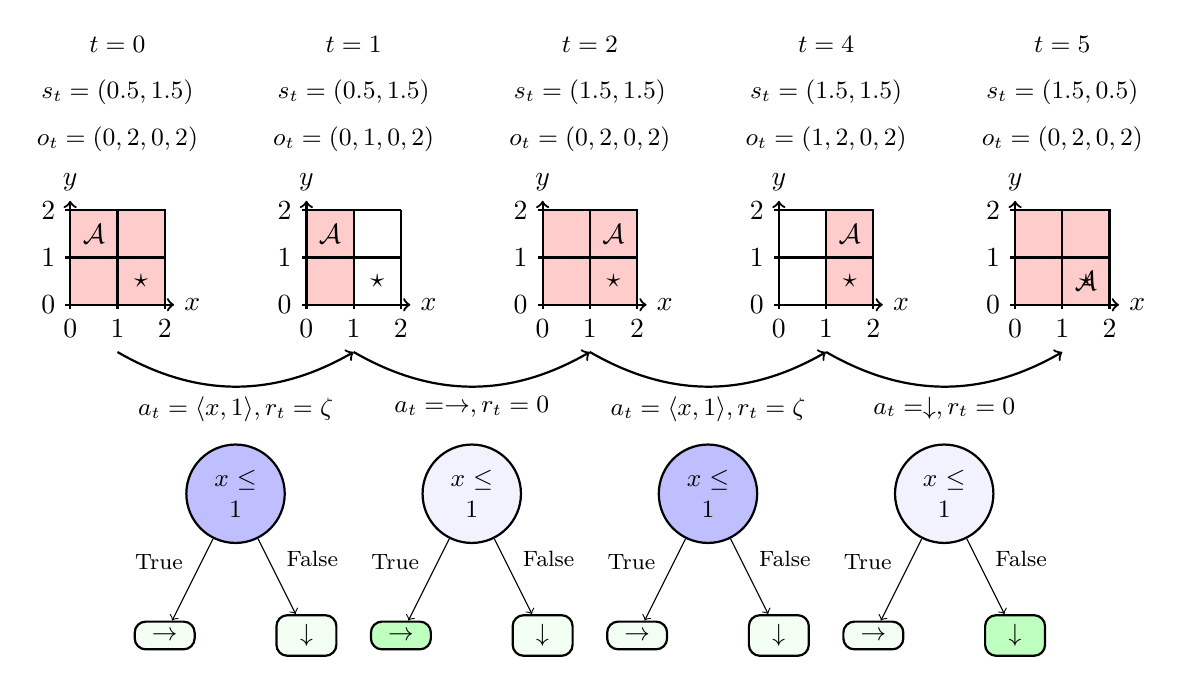
\begin{tikzpicture}[scale=0.6]
    % Define styles
    \tikzstyle{grid}=[draw, thick, fill=gray!10]
    \tikzstyle{rectangle}=[draw, thick, fill=red!20]
    
    % Row 1: IBMDP States (s, o)
    % t=0: Initial state
    \node at (2,9.5) {\small $t=0$};
    \node at (2,8.5) {\small $\boldsymbol{s}_t=(0.5, 1.5)$};
    \node at (2,7.5) {\small $\boldsymbol{o}_t=(0, 2, 0, 2)$};

    \draw[rectangle] (1,4) rectangle (3,6);
    \draw[grid] (1,4) grid (3,6);
    % Add axes
    \draw[thick, ->] (1,4) -- (3.2,4) node[right] {$x$};
    \draw[thick, ->] (1,4) -- (1,6.2) node[above] {$y$};
    \foreach \x in {0,1,2} {
        \draw[thick] (\x+1,4) -- (\x+1,3.9) node[below] {$\x$};
    }
    \foreach \y in {0,1,2} {
        \draw[thick] (1,\y+4) -- (0.9,\y+4) node[left] {$\y$};
    }
    \node at (1.5, 5.5) {$\mathcal{A}$};
    \node at (2.5, 4.5) {$\star$};
    
    % Curved arrow from t=0 to t=1
    \draw[thick, ->] (2,3) to[bend right=30] node[midway, below] {\small $a_t = \langle x, 1\rangle, r_t = \zeta$} (7,3);

    % % t=1: After AIG x≤0.5
    \node at (7,9.5) {\small $t=1$};
    \node at (7,8.5) {\small $\boldsymbol{s}_t=(0.5, 1.5)$};
    \node at (7,7.5) {\small $\boldsymbol{o}_t=(0, 1, 0, 2)$};

    \draw[rectangle] (6,4) rectangle (7,6);
    \draw[grid] (6,4) grid (8,6);
    % Add axes
    \draw[thick, ->] (6,4) -- (8.2,4) node[right] {$x$};
    \draw[thick, ->] (6,4) -- (6,6.2) node[above] {$y$};
    \foreach \x in {0,1,2} {
        \draw[thick] (\x+6,4) -- (\x+6,3.9) node[below] {$\x$};
    }
    \foreach \y in {0,1,2} {
        \draw[thick] (6,\y+4) -- (5.9,\y+4) node[left] {$\y$};
    }
    \node at (6.5, 5.5) {$\mathcal{A}$};
    \node at (7.5, 4.5) {$\star$};


    % Curved arrow from t=1 to t=2
    \draw[thick, ->] (7,3) to[bend right=30] node[midway, below] {\small $a_t = \rightarrow, r_t  = 0$}(12,3);

    \node[circle, draw, thick, fill=blue!25, text width=2em, text centered, minimum height=1.5em, font=\small] (tree4_root) at (4.5,0) {$x \leq 1$};
    \node[rectangle, draw, thick, fill=green!5, text width=1.5em, text centered, rounded corners, minimum height=1em, font=\small] (tree4_right) at (3,-3) {$\rightarrow$};
    \node[rectangle, draw, thick, fill=green!5, text width=1.5em, text centered, rounded corners, minimum height=1em, font=\small] (tree4_left) at (6,-3) {$\downarrow$};
    \draw[->] (tree4_root) -- (tree4_right) node[font=\footnotesize, midway, above left] {True};
    \draw[->] (tree4_root) -- (tree4_left) node[font=\footnotesize, midway, above right] {False};

    \node at (12,9.5) {\small $t=2$};
    \node at (12,8.5) {\small $\boldsymbol{s}_t=(1.5, 1.5)$};
    \node at (12,7.5) {\small $\boldsymbol{o}_t=(0, 2, 0, 2)$};
    
    \draw[rectangle] (11,4) rectangle (13,6);
    \draw[grid] (11,4) grid (13,6);
    % Add axes
    \draw[thick, ->] (11,4) -- (13.2,4) node[right] {$x$};
    \draw[thick, ->] (11,4) -- (11,6.2) node[above] {$y$};
    \foreach \x in {0,1,2} {
        \draw[thick] (\x+11,4) -- (\x+11,3.9) node[below] {$\x$};
    }
    \foreach \y in {0,1,2} {
        \draw[thick] (11,\y+4) -- (10.9,\y+4) node[left] {$\y$};
    }
    \node at (12.5, 5.5) {$\mathcal{A}$};
    \node at (12.5, 4.5) {$\star$};
    
    % Curved arrow from t=2 to t=4
    \draw[thick, ->] (12,3) to[bend right=30] node[midway, below] {\small $a_t = \langle x, 1 \rangle, r_t = \zeta$} (17,3);

    \node[circle, draw, thick, fill=blue!5, text width=2em, text centered, minimum height=1.5em, font=\small] (tree4_root) at (9.5,0) {$x \leq 1$};
    \node[rectangle, draw, thick, fill=green!25, text width=1.5em, text centered, rounded corners, minimum height=1em, font=\small] (tree4_right) at (8,-3) {$\rightarrow$};
    \node[rectangle, draw, thick, fill=green!5, text width=1.5em, text centered, rounded corners, minimum height=1em, font=\small] (tree4_left) at (11,-3) {$\downarrow$};
    \draw[->] (tree4_root) -- (tree4_right) node[font=\footnotesize, midway, above left] {True};
    \draw[->] (tree4_root) -- (tree4_left) node[font=\footnotesize, midway, above right] {False};

    
    \node at (17,9.5) {\small $t=4$};
    \node at (17,8.5) {\small $\boldsymbol{s}_t=(1.5, 1.5)$};
    \node at (17,7.5) {\small $\boldsymbol{o}_t=(1, 2, 0, 2)$};

    \draw[rectangle] (17,4) rectangle (18,6);
    \draw[grid] (16,4) grid (18,6);
    % Add axes
    \draw[thick, ->] (16,4) -- (18.2,4) node[right] {$x$};
    \draw[thick, ->] (16,4) -- (16,6.2) node[above] {$y$};
    \foreach \x in {0,1,2} {
        \draw[thick] (\x+16,4) -- (\x+16,3.9) node[below] {$\x$};
    }
    \foreach \y in {0,1,2} {
        \draw[thick] (16,\y+4) -- (15.9,\y+4) node[left] {$\y$};
    }
    \node at (17.5, 5.5) {$\mathcal{A}$};
    \node at (17.5, 4.5) {$\star$};
    
    \draw[thick, ->] (17,3) to[bend right=30] node[midway, below] {\small $a_t = \downarrow, r_t = 0$} (22,3);
    
    \node[circle, draw, thick, fill=blue!25, text width=2em, text centered, minimum height=1.5em, font=\small] (tree4_root) at (14.5,0) {$x \leq 1$};
    \node[rectangle, draw, thick, fill=green!5, text width=1.5em, text centered, rounded corners, minimum height=1em, font=\small] (tree4_right) at (13,-3) {$\rightarrow$};
    \node[rectangle, draw, thick, fill=green!5, text width=1.5em, text centered, rounded corners, minimum height=1em, font=\small] (tree4_left) at (16,-3) {$\downarrow$};
    \draw[->] (tree4_root) -- (tree4_right) node[font=\footnotesize, midway, above left] {True};
    \draw[->] (tree4_root) -- (tree4_left) node[font=\footnotesize, midway, above right] {False};


    \node at (22,9.5) {\small $t=5$};
    \node at (22,8.5) {\small $\boldsymbol{s}_t=(1.5, 0.5)$};
    \node at (22,7.5) {\small $\boldsymbol{o}_t=(0, 2, 0, 2)$};
 
    \draw[rectangle] (21,4) rectangle (23,6);
    \draw[grid] (21,4) grid (23,6);
    % Add axes
    \draw[thick, ->] (21,4) -- (23.2,4) node[right] {$x$};
    \draw[thick, ->] (21,4) -- (21,6.2) node[above] {$y$};
    \foreach \x in {0,1,2} {
        \draw[thick] (\x+21,4) -- (\x+21,3.9) node[below] {$\x$};
    }
    \foreach \y in {0,1,2} {
        \draw[thick] (21,\y+4) -- (20.9,\y+4) node[left] {$\y$};
    }
    \node at (22.5, 4.5) {$\mathcal{A}$};
    \node at (22.5, 4.5) {$\star$};

    \node[circle, draw, thick, fill=blue!5, text width=2em, text centered, minimum height=1.5em, font=\small] (tree4_root) at (19.5,0) {$x \leq 1$};
    \node[rectangle, draw, thick, fill=green!5, text width=1.5em, text centered, rounded corners, minimum height=1em, font=\small] (tree4_right) at (18,-3) {$\rightarrow$};
    \node[rectangle, draw, thick, fill=green!25, text width=1.5em, text centered, rounded corners, minimum height=1em, font=\small] (tree4_left) at (21,-3) {$\downarrow$};
    \draw[->] (tree4_root) -- (tree4_right) node[font=\footnotesize, midway, above left] {True};
    \draw[->] (tree4_root) -- (tree4_left) node[font=\footnotesize, midway, above right] {False};

    
\end{tikzpicture}
\caption{An IBMDP trajectory when the base MDP is 2$\times$2 grid world. In the top row, we write the visited base state features and observations, in the middle row, we graphically represent those, and in the bottom row, we present the corresponding decision tree policy traversal.
$\mathcal{A}$ tracks the current state features $\boldsymbol{s}_t$ in the grid.
The pink obstructions of the grid represent the current observations $\boldsymbol{o}_t$ of the base state features.
When the pink covers the whole grid, the information contained in the observation could be interpreted as ``the current state features could be anywhere in the grid''.
The more information gathering actions are taken, the more refined the bounds on the current base state features get.
At $t=0$, the base state features are $\boldsymbol{s}_0 = (0.5, 1.5)$. 
The initial observation is always the base MDP default state feature bounds, here $\boldsymbol{o}_0=(0, 2, 0, 2)$ because the base state features are in $[0, 2] \times [0, 2]$.
This means that the IBMDP state is $\boldsymbol{s}_{IB} = (0.5, 1.5, 0, 2, 0, 2)$.
The first action is an IGA $\langle x, 1\rangle$ that tests the feature $x$ of the base state against the value $1$ and the reward $\zeta$. 
This transition corresponds to going through an internal node $ x\leq 1$ in a decision tree policy as illustrated in the figure. 
At $t=1$, after gathering the information that the $x$-value of the current base state is below 1, the observation is updated with the refined bounds $\boldsymbol{o}_1=(0, 1, 0, 2)$, i.e. the pink area shrinks, and the base state features remain unchanged.
The agent then takes a base action that is to move right. 
This gives a reward 0, resets the observation to the original base state feature bounds, and changes the features to $\boldsymbol{s}_2=(1.5, 1.5)$. And the trajectory continues like this until the absorbing base state $\boldsymbol{s}_5=(1.5, 0.5)$ is reached.}
\label{example:ibmdp}
\end{figure}

\section{Summary}
In this chapter, we presented the approach of Topin et. al.~\cite{topin2021iterative} to find decision tree policies that directly trade off interpretability and the RL objective rather than a surrogate imitation loss.
In particular, Topin et. al. showed that deterministic partially observable policies for iterative bounding Markov decision processes are decision tree policies for MDPs (cf. definitions~\ref{def:ibmdp} and \ref{def:po-policy}, algorithm~\ref{alg:extract-tree}, and example~\ref{example:ibmdp}).

The great promise of Topin et. al. is that one can use any reinforcement learning algorithm, e.g. PPO or DQN (cf. section~\ref{sec:drl}), to learn deterministic partially observable policies. Indeed, such policies can be encoded as e.g. neural networks as long as they satisfy proposition~\ref{def:po-policy}: this circumvents the non-differentiability limitations in direct learning of non-parametric decision tree policies.
Once a deterministic partially observable policy is obtained, a decision tree policy that trades off naturally, the RL objective in the base MDP and, interpretability through the additional reward signal $\zeta$ (cf. definition~\ref{def:ibmdp}), can be extracted with algorithm~\ref{alg:extract-tree}.
We define an interpretable RL objective as follows:
\begin{definition}[Interpretable RL objective]\label{def:irl}
    Given a base MDP $\mathcal{M} \langle S, A, R, T, T_0 \rangle$ for which we want an interpretable policy, e.g. a decision tree, a discount factor $\gamma \in (0,1]$, some interpretability penalty $\zeta$, and a set of information gathering actions $A_{info}$, the objective is to find a deterministic partially observable policy $\pi_{po}: O \rightarrow A\cup A_{info}$ (cf. definition~\ref{def:po-policy}) that maximizes:
\begin{align*}
    \mathbb{E}\left[\sum_{t=0}^{\infty} \gamma^t R((\boldsymbol{s}_t, \boldsymbol{o}_t), a_t) \mid \boldsymbol{s}_0 \sim T_0, a_t = \pi_{po}(\boldsymbol{o}_t), \boldsymbol{s}_{t+1} \sim T(\boldsymbol{s}_t, a_t), \boldsymbol{o}_{t+1}\sim T(\boldsymbol{o_t}, a_t)\right]\\
    = \mathbb{E}[V^{\pi_{po}}(\boldsymbol{s}_0, \boldsymbol{o}_0)| \boldsymbol{s}_0\sim T_0]
\end{align*}
With $V^{\pi_{po}}$ the value function (cf. definition~\ref{def:vs}) of $\pi_{po}$ in the IBMDP $\mathcal{M}_{IB}$ $\langle S \times O,A \cup A_{info}, (R, \zeta), (T_{info}, T, T_0)\rangle$ (cf. definition~\ref{def:ibmdp}).
\end{definition}

After optimizing objective with, e.g. reinforcement learning (cf. section~\ref{sec:rl}), we can use algorithm~\ref{alg:extract-tree} to obtain a decision tree policy that trades off between interpretability and the RL objective for the base MDP of interest.
This is exactly what we do in the next chapters.
% In figure (\ref{fig:summary-ibmdp}) we summarize the direct reinforcement learning approach of Topin et. al. that we use in the next chapters. 
% \begin{figure}
%     \centering
%     \begin{tikzpicture}
%         \draw[fill=blue!30] (0, 0) rectangle (5.9, 3);
%         \node at (3, 2.5) {IBMDP $\mathcal{M}_{IB} \langle \mathcal{M}, O, A_{info}, \zeta, T_{info}\rangle$};
%         \draw[fill=blue!10] (0, 0) rectangle (5, 2);
%         \node at (3, 1.5) {MDP $\mathcal{M} \langle S, A, R, T, T_0 \rangle$};
        
%         \draw[fill=red!10] (10, 0) rectangle (14, 3);
%         \node at (12, 2) {\textbf{Objective}};
%         \node at (12, 1) {$\pi^{\star}_{po} = \underset{\pi_{po}}{\operatorname{argmax}} \mathbb{E}[V^{\pi_{po}}(\boldsymbol{s}_0, \boldsymbal{o}_0)| \boldsymbol{s}_0\sim T_0]$};
        
%         \draw[fill=red!10] (1, -5) rectangle (5, -2);
%         \node at (3, -3) {\textbf{Decision Tree Policy}};
%         \node at (3, -4) {$\pi_{\mathcal{T}}: S \rightarrow A$};
        
%         \draw[fill=red!10] (9.5, -5) rectangle (14.5, -2);
%         \node at (12, -3) {\textbf{Deterministic Policy}};
%         \node at (12, -4) {$\pi_{po}: O \rightarrow A \cup A_{info}$};
        
%         \draw[thick, ->] (6, 2) -- (10, 2) node[midway, above] {$\gamma$};
%         \draw[thick, <-] (5, -3.5) -- (9.5, -3.5) node[midway, above] {Extract tree with Alg 6};
%         \draw[thick, ->] (12, 0) -- (12, -2) node[midway, left] {Solve with e.g. RL};
%         \draw[thick, <-] (3, 0.5) -- (3, -2) node[midway, left] {Can be interpreted};
    
        
%         % % Final arrow from tree back to base MDP - adjusted position
%         % \draw[thick, ->] (1.75, -2.5) -- (1.75, -0.5) node[midway, right] {Can deploy\\and interpret};
        
%     \end{tikzpicture}
%     \caption{A formal framework to learn decision tree policies for MDPs. This include learning a deterministic partially observable policy in a POIBMDP (cite).}
%     \label{fig:summary-ibmdp}
%     \end{figure}

